\documentclass{article}

% Packages
\usepackage[utf8]{inputenc} % For modern characters
\usepackage{microtype} % For sexy kerning
\usepackage{mathtools} % For math stuff
\usepackage{amssymb} % For math symbols
\usepackage{tabularx} % For making tables
\usepackage{fancyhdr} % Use a header
%\usepackage{fullpage} % Get rid of white space in margins
% fullpage package doesn't work with fancyhdr

% Set the margins
\usepackage[scale=0.8, top=1in, bottom=1in]{geometry}

% Other front matter
\newcommand{\code}[1]{\texttt{#1}} % More readable for writing inline code.
\newcommand{\p}[1]{\paragraph{#1}} % Easier to type out for paragraph command
\newcommand{\tab}{\hspace*{3em}} % Set tab spaces
\pagestyle{fancy} % Makes Header Possible
{ %%% Header Set up
	\lhead{} % Set the left header to be blank
	\chead{} % Set the center header to be blank
	% Header for every page except the first two
	\rhead{Ben Foster | Lab 4 | May 7, 2015} % Name, assignment, date
}
\setcounter{tocdepth}{2} % Set Table of Contents Depth
\setlength{\parindent}{0pt} % Disable automatic indentation

%%%%%%%%%%%%%%%%%%%% Begin Document %%%%%%%%%%%%%%%%%%%%
\begin{document}

{ % Title page, table of contents, and page number setting
	\title{Probability and Statistics for Engineers Lab Four \\ TMATH 390}
	\author{Ben Foster\thanks{
		Institute of Technology, University of Washington Tacoma} \\
		Instructor: Julia Eaton}
	\date{May 7, 2015}
	\maketitle
	\thispagestyle{empty} % No page number at bottom
	\clearpage
	
	\pagenumbering{roman}
	\tableofcontents
	\clearpage
	\setcounter{page}{1}
	\pagenumbering{arabic}
}

\section*{First Printout}
\addcontentsline{toc}{section}{First Printout}

%\begin{figure}[!htbp]
\begin{center}
   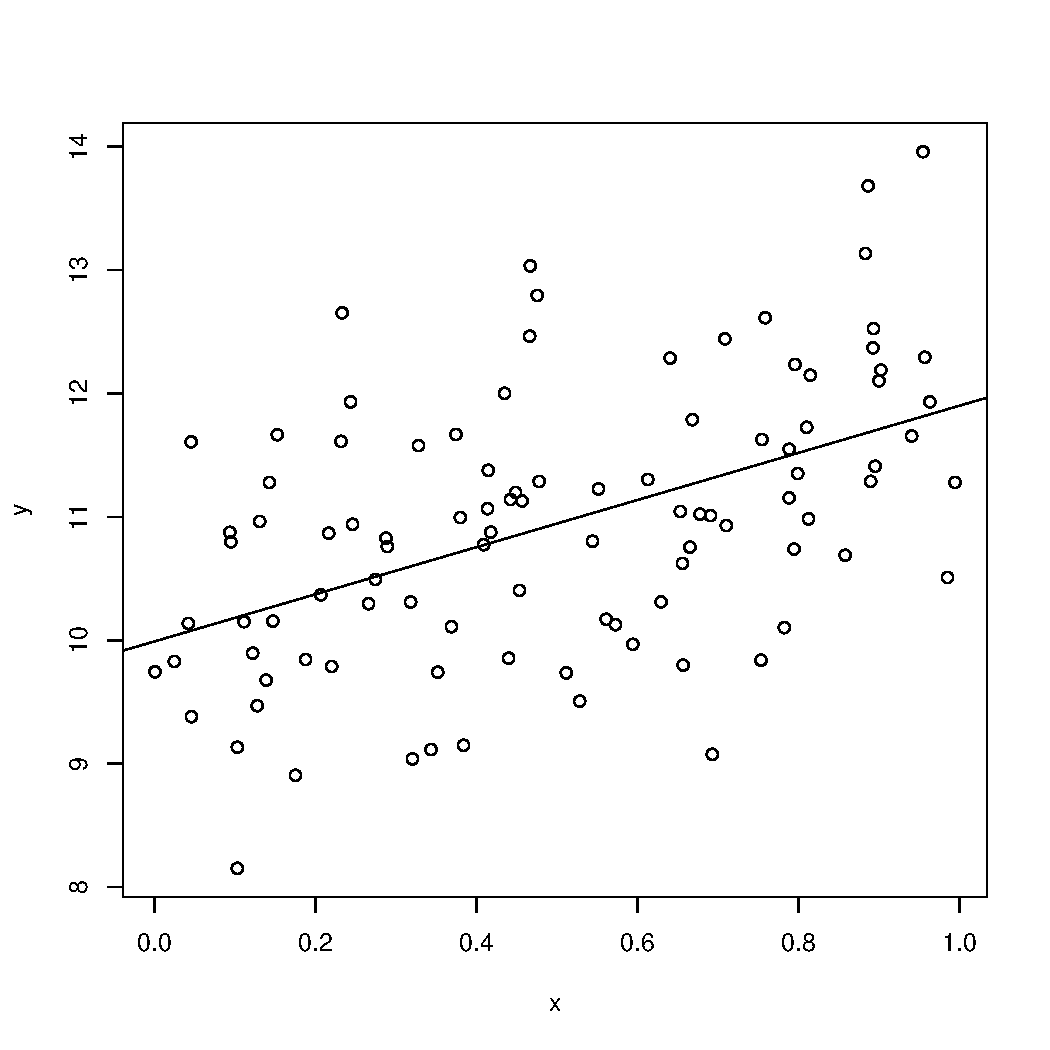
\includegraphics[width=\textwidth]{img/Lab4_print_1.pdf} 
\end{center}
%   \caption{Regression on fake/simulated data}
%   \label{fig:print_1}
%\end{figure}

\section*{Second Printout}
\addcontentsline{toc}{section}{Second Printout}

\begin{center}
   \includegraphics[width=\textwidth]{img/Lab4_print_2.pdf} 
\end{center}

%\vspace{-30pt}
%\begin{figure}[!htbp]
%   \centering
%   \includegraphics[width=4in]{Lab4_print_2.pdf} 
%   \caption{Regression on real (hail) data}
%   \label{fig:print_2}
%\end{figure}

\section*{Third Printout}
\addcontentsline{toc}{section}{Third Printout}

\begin{center}
   \includegraphics[width=\textwidth]{img/Lab4_print_3.pdf} 
\end{center}

%\begin{figure}[!htbp]
%   \centering
%   \includegraphics[width=4in]{Lab4_print_3.pdf} 
%   \caption{Visual assessment of goodness-of-fit}
%   \label{fig:print_3}
%\end{figure}

\clearpage
\section*{Lab Exercise}
\addcontentsline{toc}{section}{Lab Exercise}

Here is some data: \\

\begin{tabular}{ l l l l l }
	$x$: & 0 & 2 & 4 & 6 \\
	$y$: & 1 & 7 & 55 & 400 \\
\end{tabular} \\

(a) What is the value of $R^2$ for a line through this data? \\
(b) Give one reason for why this value of $R^2$ is not very high (e.g., 0.9) \\

Turn in both parts along with the plots asked for. \\
For part (a), give me the code you typed to produce $R^2$ along with the value.

\p{Answer to part a}
In order to find $R^2$, all we have to do is input the command \code{summary(lm(y $\sim$ x))} which will give us an $R^2$ value of 0.7079.

\p{Answer to part b}
The value of $R^2$, while still pretty high, is not extremely high mainly because of the extreme outlier (6,400) all the way up in the corner of the graph. If it weren't for this point, then our $R^2$ value would be higher along with our $r$ value. It could also be because we don't have that many data points, and so extreme outliers have a much greater effect on $R^2$.

\begin{figure}[!htbp]
   \centering
   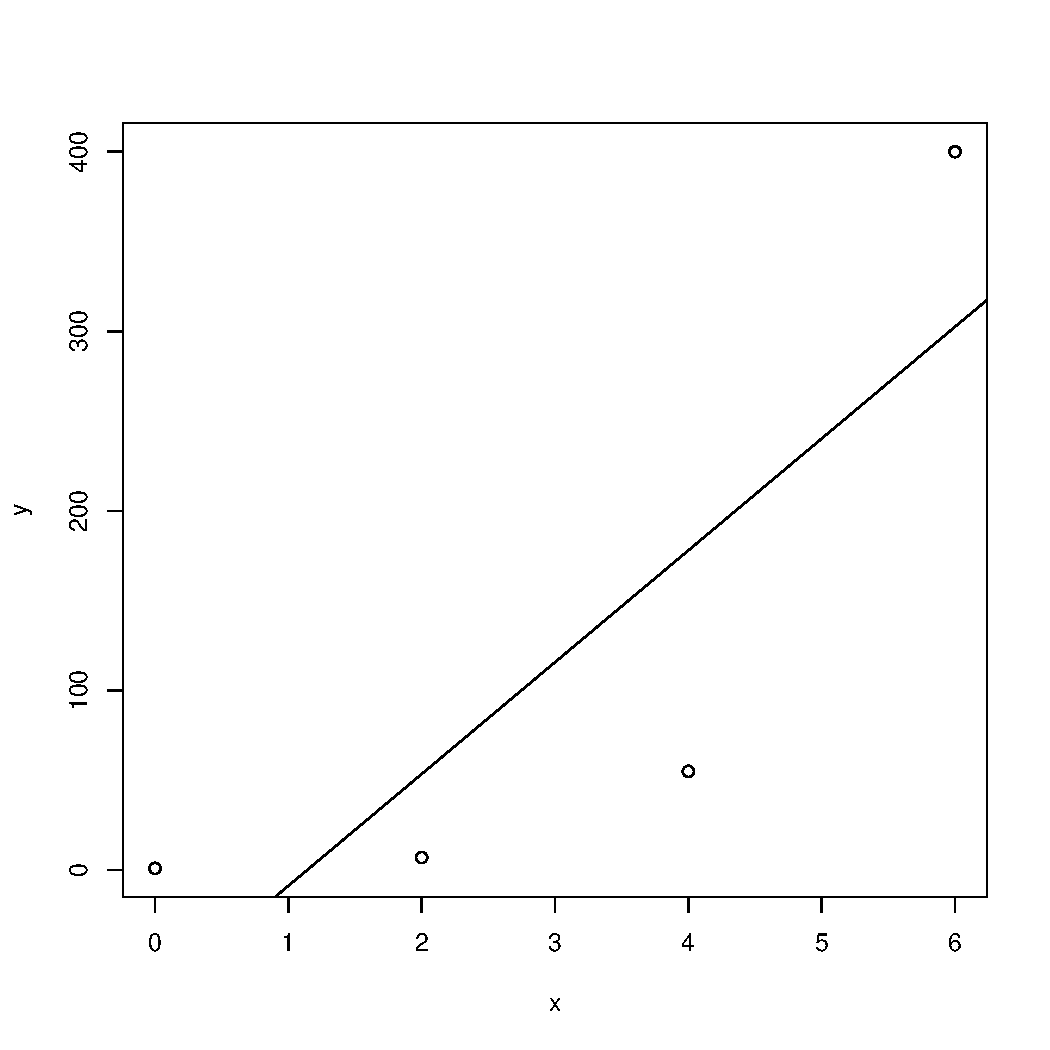
\includegraphics[width=5in]{img/Lab4_print_4.pdf} 
   \caption{Lab Exercise}
   \label{fig:print_4}
\end{figure}

\end{document}